\documentclass[conference]{IEEEtran}
\IEEEoverridecommandlockouts

\usepackage{cite}
\usepackage{amsmath,amssymb,amsfonts}
\usepackage{algorithm}
\usepackage{algorithmic}
\usepackage{graphicx}
\usepackage{textcomp}
\usepackage{xcolor}
\usepackage{booktabs}
\usepackage{tabularx}
\usepackage{array}
\usepackage{url}
\usepackage{balance}
\usepackage{tikz}
\usetikzlibrary{arrows.meta}

\def\BibTeX{{\rm B\kern-.05em{\sc i\kern-.025em b}\kern-.08em
    T\kern-.1667em\lower.7ex\hbox{E}\kern-.125emX}}

\begin{document}

\title{VISHWAAS: Approval-First VPN Management\\with Human Oversight and Layered Access Control}

\author{
  \IEEEauthorblockN{Anurag Krishna Sharma, HariOm Prakash, Anitha Naidu, J Jayachandran}
  \IEEEauthorblockA{
    \textit{NSED} \\
    \textit{Advanced Data Processing Research Institute} \\
  }
}

\maketitle

% ─────────────────────────────────────────────────────────────────────────────
\begin{abstract}
Deploying WireGuard across a group of machines typically requires
either manually editing configuration files on every machine or
relying on automated peer-exchange tools that connect nodes without
any human review. Neither approach is satisfactory in environments
where network access decisions must be deliberate and traceable.
This paper describes the design and implementation of VISHWAAS
(\textit{Sanskrit: ``trust''}), a self-hosted VPN management platform
that places an explicit administrator approval step in front of every
network change. No machine joins the VPN and no peer connection
becomes active without a human decision recorded in an audit log.
A central controller with a web dashboard manages all state; a
lightweight agent on each machine translates approved decisions
into live WireGuard configuration automatically. We describe the
overall system design, the enrollment and peering workflows, the
three-tier key management model including optional TPM hardware
binding, the layered security controls, and lessons from deploying
the system on a three-machine internal lab network.
\end{abstract}

\begin{IEEEkeywords}
WireGuard, VPN orchestration, human-in-the-loop, network access control,
TPM~2.0, audit logging, FastAPI, self-hosted
\end{IEEEkeywords}


% =============================================================================
\section{Introduction}
% =============================================================================

WireGuard~\cite{donenfeld2017wireguard} has become a popular choice for
building VPN tunnels because of its small codebase, strong cryptography,
and high throughput. However, WireGuard is a low-level primitive. It manages
encrypted tunnels but provides no mechanism for deciding who is allowed to
join a network, how keys are distributed, or how connections between nodes
are authorised. Operators fill this gap in one of two ways.

The first approach is static configuration: an administrator writes
\texttt{wg-quick} files by hand and copies them to every machine. This is
error-prone, hard to update across many nodes, and leaves no record of
\textit{why} a particular peer relationship exists or who created it.

The second approach is automated coordination: a daemon handles peer
discovery and key exchange without human involvement. This is easy to
operate but gives up the ability to review or audit individual network
access decisions.

Our lab needed a third option---one where WireGuard configuration is still
automated (no manual SSH) but every network change requires an explicit
human decision. We built VISHWAAS to fill this gap. The system's design
centres on a single invariant: \emph{no node joins the VPN and no peer
connection becomes active unless an administrator has clicked Approve}.
All decisions are stored in an append-only log so the history of every
network change is always available.

\subsection{Design Goals}

The system was built against five concrete goals:

\begin{enumerate}
  \item \textbf{Explicit approval}: every join and every connection requires a
        positive admin action; automated approval is not possible.
  \item \textbf{Audit trail}: every state change produces an immutable log
        entry with a timestamp and event type.
  \item \textbf{Zero-touch provisioning}: once approved, WireGuard is
        configured on the relevant machines automatically---no SSH, no file
        editing.
  \item \textbf{Flexible key security}: support disk-based, controller-issued,
        and TPM hardware-bound key storage on the same codebase.
  \item \textbf{No public API exposure}: neither the controller management API
        nor the per-node agent API should be reachable from the internet.
\end{enumerate}


% =============================================================================
\section{Background and Motivation}
\label{sec:background}
% =============================================================================

\subsection{WireGuard Fundamentals}

WireGuard~\cite{donenfeld2017wireguard} is a Layer-3 VPN protocol built
into the Linux kernel. It uses Curve25519 for key agreement,
ChaCha20-Poly1305 for authenticated encryption, and BLAKE2s for hashing.
Every peer is identified by a 256-bit public key. Routing is governed by
per-peer \texttt{allowed-ips} rules. There are no certificates, no CAs,
and no negotiation phase. WireGuard itself is intentionally minimal;
all peer management and key distribution must be handled externally.

\subsection{Why Existing Tools Did Not Fit}

\textbf{Tailscale}~\cite{tailscale} automates peer discovery and connection
via a cloud coordination server. Nodes join after a single authentication
step. Approval is per-device, not per-connection, and the coordination server
is hosted by Tailscale rather than the operator. For an internal deployment
where the operator must control all state locally, this was not suitable.

\textbf{Nebula}~\cite{nebula} distributes certificates at deployment time and
uses lighthouse nodes for peer discovery. Like static WireGuard configurations,
it provides no runtime approval step. A new peer relationship cannot be
reviewed before it becomes active.

\textbf{Ansible and Terraform} WireGuard roles provision configuration
reproducibly but are push-based tools run at deployment time. They cannot
respond to a machine coming online mid-deployment without re-running the
full playbook. We needed a persistent control loop.

VISHWAAS is designed specifically for the case where the operator wants
to keep a WireGuard-based network but needs a running approval workflow
and a complete activity history---neither of which the above tools provide
out of the box.


% =============================================================================
\section{System Design}
\label{sec:architecture}
% =============================================================================

VISHWAAS is split into two components: a \textbf{controller} that runs on
one central machine and an \textbf{agent} that runs on every VPN node.

\begin{figure}[!t]
\centering
\resizebox{\columnwidth}{!}{%
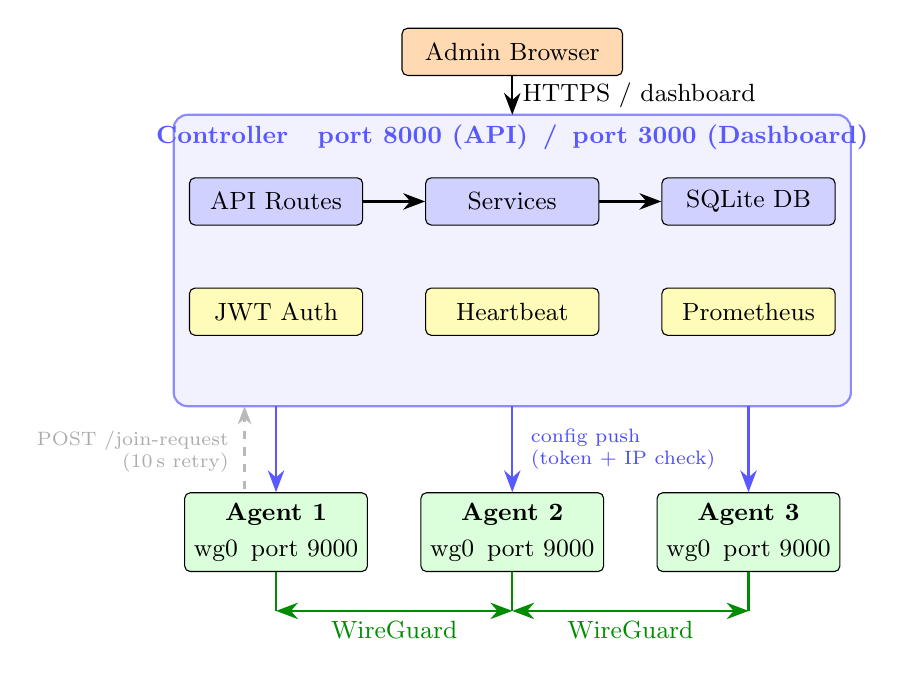
\begin{tikzpicture}[
  box/.style={draw, rectangle, rounded corners=2pt,
              text centered, align=center,
              minimum height=0.6cm, minimum width=2.2cm,
              font=\small},
  arr/.style={-{Stealth[scale=1.2]}, thick},
  wgarr/.style={{Stealth[scale=1.2]}-{Stealth[scale=1.2]}, thick, green!55!black}
]

% ── Admin browser ──
\node[box, fill=orange!30, minimum width=2.8cm] (admin) at (4.5, 7.0)
     {Admin Browser};

% ── Controller bounding box ──
\filldraw[draw=blue!45, thick, rounded corners=5pt, fill=blue!5]
     (0.2, 2.5) rectangle (8.8, 6.2);
\node[font=\small\bfseries, text=blue!65, anchor=north] at (4.5, 6.2)
     {Controller\quad port~8000 (API)\enspace /\enspace port~3000 (Dashboard)};

% ── Logic row ──
\node[box, fill=blue!18] (api) at (1.5, 5.1) {API Routes};
\node[box, fill=blue!18] (svc) at (4.5, 5.1) {Services};
\node[box, fill=blue!18] (db)  at (7.5, 5.1) {SQLite DB};

% ── Infrastructure row ──
\node[box, fill=yellow!28] (jwt)  at (1.5, 3.7) {JWT Auth};
\node[box, fill=yellow!28] (hb)   at (4.5, 3.7) {Heartbeat};
\node[box, fill=yellow!28] (prom) at (7.5, 3.7) {Prometheus};

% ── Internal flow ──
\draw[arr] (api) -- (svc);
\draw[arr] (svc) -- (db);

% ── Agents  (center y=0.9, min-height=1.0cm → north=1.4, south=0.4) ──
\node[box, fill=green!14, minimum height=1.0cm, minimum width=2.2cm]
     (ag1) at (1.5, 0.9) {\textbf{Agent 1}\\[2pt]wg0\enspace port~9000};
\node[box, fill=green!14, minimum height=1.0cm, minimum width=2.2cm]
     (ag2) at (4.5, 0.9) {\textbf{Agent 2}\\[2pt]wg0\enspace port~9000};
\node[box, fill=green!14, minimum height=1.0cm, minimum width=2.2cm]
     (ag3) at (7.5, 0.9) {\textbf{Agent 3}\\[2pt]wg0\enspace port~9000};

% ── Admin → controller ──
\draw[arr] (admin.south) --
     node[right, font=\small] {HTTPS / dashboard} (4.5, 6.2);

% ── Controller → agents: blue config-push arrows ──
\draw[arr, blue!65] (1.5, 2.5) -- (ag1.north);
\draw[arr, blue!65] (4.5, 2.5) --
     node[right=3pt, font=\scriptsize, text=blue!70, align=left, pos=0.5]
     {config push\\(token + IP check)} (ag2.north);
\draw[arr, blue!65] (7.5, 2.5) -- (ag3.north);

% ── Join request: agents → controller (dashed gray, offset left of blue arrows) ──
\draw[-{Stealth[scale=1.0]}, thick, gray!55, dashed]
     (1.1, 1.45) --
     node[left=2pt, font=\scriptsize, text=gray!65, align=right, pos=0.45]
     {POST /join-request\\(10\,s retry)}
     (1.1, 2.5);

% ── WireGuard tunnels: drop below each agent box, then bidirectional
%    south=0.4, drop 0.5 → horizontal rail at y=−0.1 ──
\draw[green!55!black, thick] (ag1.south) -- ++(0, -0.5);
\draw[green!55!black, thick] (ag2.south) -- ++(0, -0.5);
\draw[green!55!black, thick] (ag3.south) -- ++(0, -0.5);
\draw[wgarr] (1.5, -0.1) -- node[below, font=\small] {WireGuard} (4.5, -0.1);
\draw[wgarr] (4.5, -0.1) -- node[below, font=\small] {WireGuard} (7.5, -0.1);

\end{tikzpicture}}
\caption{VISHWAAS system architecture. Communication is asymmetric: agents
initiate enrollment via \texttt{POST /join-request} (dashed arrow), but all
subsequent configuration commands flow controller-to-agent only (blue solid
arrows), authenticated by token and restricted to the management LAN.
After provisioning, nodes communicate directly over encrypted tunnels
(green), bypassing the controller entirely.}
\label{fig:architecture}
\end{figure}

Communication is asymmetric. Agents send join requests to the controller.
The controller sends all configuration commands to agents. After a connection
is approved, WireGuard traffic flows directly between nodes and does not
pass through the controller.

\subsection{Controller}

The controller is a FastAPI backend paired with a React single-page
dashboard. Internally it is organised into:

\begin{itemize}
  \item \textbf{API Routes}: HTTP endpoints with Pydantic input validation
        and per-route rate limiting.
  \item \textbf{Services}: Business logic for enrollment, connection approval,
        and agent communication. This layer is intentionally stateless.
  \item \textbf{Persistence}: SQLAlchemy ORM with a SQLite database recording
        every node, request, connection, and log event.
  \item \textbf{Domain}: Python enumerations for every valid status value,
        preventing illegal state transitions at the type level.
  \item \textbf{Core}: Configuration loaded from environment variables,
        JWT utilities, a background heartbeat task, Prometheus metrics, and
        correlation ID middleware.
\end{itemize}

All HTTP calls from the controller to agents share a single \texttt{httpx}
connection pool. Failed calls are retried with exponential backoff (2 retries
at 1\,s and 2\,s delays). A correlation ID is forwarded to every agent call
to allow end-to-end request tracing in logs.

\subsection{Agent}

The agent is a small FastAPI service whose entire job is to translate
controller commands into WireGuard kernel calls. Its components are:

\begin{itemize}
  \item \textbf{Main}: Startup logic, the background join-retry loop, and
        all HTTP endpoint handlers.
  \item \textbf{WireGuard}: Thin wrappers around the \texttt{wg} and
        \texttt{ip} CLI tools, providing idempotent \texttt{provision\_interface},
        \texttt{add\_peer}, and \texttt{remove\_peer} operations.
  \item \textbf{State}: A four-state machine (\texttt{WAITING},
        \texttt{APPROVED}, \texttt{ACTIVE}, \texttt{ERROR}) persisted to a
        JSON file on disk so the agent survives process restarts without
        losing its current status.
  \item \textbf{Security}: \texttt{ControllerIPMiddleware} checks the source
        IP of every incoming request against a configured allowlist. Requests
        from any other IP return HTTP~403 before reaching any route handler.
  \item \textbf{TPM}: Optional key storage in TPM~2.0 Non-Volatile memory.
\end{itemize}

\subsection{Data Model}

All controller state lives in seven SQLite tables (Table~\ref{tab:schema}).
The \texttt{logs} table is the most important from an auditability standpoint:
it is append-only by design---no service code ever updates or deletes a log
entry. The \texttt{revoked\_tokens} table implements JWT logout; expired
entries are cleaned up each time the controller starts.

\begin{table}[!t]
\caption{Database Tables}
\label{tab:schema}
\centering
\small
\setlength{\tabcolsep}{4pt}
\begin{tabularx}{\columnwidth}{@{}lX@{}}
\toprule
\textbf{Table} & \textbf{Purpose and Key Columns} \\
\midrule
\texttt{nodes}               & Approved VPN nodes: name, public\_key, vpn\_ip, status, last\_seen \\
\texttt{join\_requests}      & Enrollment attempts: public\_key, agent\_url, status \\
\texttt{connection\_requests}& Admin-initiated peer requests: node\_a, node\_b, status \\
\texttt{connections}         & Active WireGuard peer relationships: node\_a, node\_b, status \\
\texttt{notifications}       & Dashboard alerts: message, is\_read \\
\texttt{logs}                & Append-only audit trail: event\_type, description, timestamp \\
\texttt{revoked\_tokens}     & JWT logout blacklist: jti, expires\_at \\
\bottomrule
\end{tabularx}
\end{table}


% =============================================================================
\section{Approval Workflows}
\label{sec:lifecycle}
% =============================================================================

\subsection{Node Enrollment}

When an agent starts up, it generates (or loads from disk) a WireGuard
keypair and enters a background loop that submits a join request to the
controller every 10 seconds. The request carries the node name, the
WireGuard public key, and the URL the controller should use to call back
to this agent.

If a request arrives with a public key that already belongs to an
existing node---meaning the agent has restarted---the controller first
tears down all active peer connections on related agents, deletes the stale
node record, and creates a fresh pending request. The administrator must
re-approve. This is a deliberate design choice: it prevents stale WireGuard
peer entries from accumulating silently after restarts.

Algorithm~\ref{alg:join_approval} specifies the approval procedure. The
node is initially recorded with status \textsc{Approved} and only becomes
\textsc{Active} once the agent confirms the WireGuard interface is up.
If the agent is temporarily unreachable at approval time, the controller
retries the provisioning push in the background.

\begin{algorithm}[!t]
\caption{Node Enrollment Approval}
\label{alg:join_approval}
\begin{algorithmic}[1]
\REQUIRE Join request $r$ with $r.\textit{status} = \textsc{Pending}$
\STATE Verify $r.\textit{status} = \textsc{Pending}$; return 409 otherwise
\STATE $\textit{vpn\_ip} \leftarrow$ next free address in $[10.10.10.2,\;10.10.10.254]$
\STATE \textbf{INSERT} node($r.\textit{name}$, $r.\textit{pubkey}$,
       $\textit{vpn\_ip}$, \textsc{Approved})
\STATE \textbf{UPDATE} $r.\textit{status} \leftarrow \textsc{Approved}$
\STATE \textbf{APPEND} log(\textsc{Join\_Approved}, timestamp)
\STATE \textbf{async}: push VPN IP to $r.\textit{agent\_url}$
\STATE \quad Retry up to 4$\times$ at 5\,s intervals on failure
\STATE \quad On ACK: \textbf{UPDATE} node.status $\leftarrow$ \textsc{Active}
\STATE \quad On all retries exhausted: node stays \textsc{Approved};
       admin may trigger manual retry from dashboard
\end{algorithmic}
\end{algorithm}

\subsection{Peer Connection}

To connect two nodes, an administrator selects them on the dashboard and
submits a connection request. The controller stores it as \textsc{Pending}
and waits for admin approval. On approval, Algorithm~\ref{alg:conn_approval}
runs. The key design property is \emph{all-or-nothing}: if configuring the
second agent fails, the first is immediately rolled back. No partial connection
state is ever written to the database.

When an administrator terminates a connection, the controller sends
peer-removal commands to both agents and marks the connection
\textsc{Terminated}. Crucially, the WireGuard interface remains up on both
machines after termination---each node keeps its VPN IP and remains reachable
on the network, it simply stops being peered with the other node.

\begin{algorithm}[!t]
\caption{Peer Connection Approval}
\label{alg:conn_approval}
\begin{algorithmic}[1]
\REQUIRE Nodes $A$, $B$; both \textsc{Active}
\STATE $r_A \leftarrow$ add-peer($A$, pubkey=$B.\textit{pk}$, endpoint=$B.\textit{url}$)
\IF{$r_A$ failed}
  \STATE \textbf{RETURN} HTTP~502 (no state written)
\ENDIF
\STATE $r_B \leftarrow$ add-peer($B$, pubkey=$A.\textit{pk}$, endpoint=$A.\textit{url}$)
\IF{$r_B$ failed}
  \STATE \textbf{ROLLBACK}: remove-peer($A$, pubkey=$B.\textit{pk}$)
  \STATE \textbf{RETURN} HTTP~502 (no state written)
\ENDIF
\STATE \textbf{INSERT} connection($A$, $B$, \textsc{Active})
\STATE \textbf{APPEND} log(\textsc{Connection\_Approved}, timestamp)
\end{algorithmic}
\end{algorithm}


% =============================================================================
\section{Cryptographic Key Handling}
\label{sec:keymanagement}
% =============================================================================

A design question that came up early was: who generates the WireGuard private
keys, and where do they live? We identified three viable strategies and
implemented all three so operators can choose based on their security
requirements. Table~\ref{tab:keymanagement} summarises the trade-offs.

\textbf{Agent-Generated (Default).} At startup the agent runs \texttt{wg
genkey} and sends only the public key in the join request. The private key
never leaves the machine. This is the simplest mode and suitable for most
deployments, but a root-level attacker can read the key directly from disk.

\textbf{Controller-Issued.} The agent sends a join request with no public
key. On approval, the controller generates a keypair, stores the public key
in the database, and delivers the private key to the agent inside the
provisioning response. This centralises key generation, making rotation
easier, but the private key travels over the wire once. TLS on the
management channel is mandatory in this mode.

\textbf{TPM Hardware-Bound.} After a keypair exists (by either strategy
above), the agent writes the private key to a TPM~2.0 Non-Volatile memory
index using \texttt{tpm2-tools}. Subsequent WireGuard calls read the key
into a short-lived temporary file and immediately delete it. The private key
never persists on the filesystem. A full disk-image dump does not yield the
key. If the TPM chip is unavailable, the system falls back to file-based
storage automatically and logs a warning.

\begin{table}[!t]
\caption{Key Management Strategy Comparison}
\label{tab:keymanagement}
\centering
\begin{tabular}{lccc}
\toprule
\textbf{Property} & \textbf{Agent-Gen} & \textbf{Ctrl-Issued} & \textbf{TPM-Bound} \\
\midrule
Private key leaves node & No  & Once & No  \\
Key persists on disk    & Yes & Yes  & No  \\
Hardware binding        & No  & No   & Yes \\
Disk-dump resistant     & No  & No   & Yes \\
Requires TPM 2.0        & No  & No   & Yes \\
Best suited for         & General & Dev/test & High-security \\
\bottomrule
\end{tabular}
\end{table}


% =============================================================================
\section{Supported Network Topologies}
\label{sec:topology}
% =============================================================================

VISHWAAS supports two routing modes controlled by an \texttt{is\_gateway}
flag on each node.

\textbf{Direct Mesh.} When no node is a gateway, each approved connection
adds a mutual \texttt{/32} peer entry on both sides, building a direct mesh.
Traffic between any two nodes takes a direct encrypted path. This works
well for small networks (up to roughly 50 nodes) but peer count grows as
$O(n^2)$.

\textbf{Hub-and-Spoke.} Marking a node as a gateway changes the routing
policy the controller pushes. A spoke node receives \texttt{allowed-ips}
$= 10.10.10.0/24$ for the gateway peer, routing all VPN traffic through the
hub. The gateway receives only a \texttt{/32} entry per spoke. The
controller also enables kernel IP forwarding on the gateway node via a
\texttt{sysctl} call to the agent. This brings peer-count complexity down to
$O(n)$ and scales to larger deployments.

Mixed configurations are supported: the controller computes the correct
\texttt{allowed-ips} for each individual connection based on the gateway
flags of both endpoints, so direct spoke-to-spoke and gateway-routed paths
can coexist in the same network.

The React dashboard renders a live force-directed graph of all
\textsc{Active} and \textsc{Approved} nodes and their connections.
\textsc{Offline} and deleted nodes are excluded so the topology view always
reflects what is actually operational.


% =============================================================================
\section{Security Model}
\label{sec:security}
% =============================================================================

\subsection{Authentication Layers}

VISHWAAS uses three distinct authentication mechanisms depending on who is
calling whom.

\textbf{Agent-to-Controller (join request).} Join requests are unauthenticated
at the transport level because the agent is, by definition, an unknown entity
at that point. Security comes from the approval gate itself: without a human
clicking Approve, the agent receives no VPN configuration. The public key in
the request acts as a cryptographic identity; a fraudulent request with a
different key receives a different IP and cannot impersonate an existing node.

\textbf{Controller-to-Agent.} Every call from the controller to an agent
endpoint carries an \texttt{X-VISHWAAS-TOKEN} header. The agent validates
this against its configured \texttt{master\_token}. A mismatch returns
HTTP~401.

\textbf{Admin dashboard.} The administrator logs in and receives a JWT
(HS256). The token carries a \texttt{jti} claim (unique token ID). Logging
out adds the \texttt{jti} to the \texttt{revoked\_tokens} table, immediately
invalidating the session regardless of the token's remaining expiry.

\subsection{Restricting API Access to Private Networks}

A recurring concern during design was that someone could call the controller
or agent APIs from the internet. We address this at two independent layers.

\textbf{Controller (nginx).} The nginx reverse proxy uses a \texttt{geo}
block to classify client IPs. RFC-1918 private addresses and loopback are
permitted; all other IPs receive HTTP~403 before the request reaches the
Python application. Health and readiness probe endpoints remain public
because monitoring systems need them.

\textbf{Agent (application layer).} The agent's
\texttt{ControllerIPMiddleware} extracts the client IP from every incoming
request and compares it against an allowlist: the controller IP (parsed from
\texttt{master\_url}), loopback, and any extras in the config file. Requests
from any other IP get HTTP~403 before any token check runs. Only the
\texttt{/health} endpoint is exempt. Because the controller is the only
legitimate caller, this completely eliminates the token brute-force attack
surface from external hosts.

\subsection{Threat Assessment}

Table~\ref{tab:threats} lists the main threats we considered during design,
the risk level, and whether VISHWAAS addresses them.

\begin{table}[!t]
\caption{Threat Assessment}
\label{tab:threats}
\centering
\small
\begin{tabularx}{\columnwidth}{lllX}
\toprule
\textbf{Threat} & \textbf{Risk} & \textbf{Status} & \textbf{Control} \\
\midrule
Rogue agent join          & Med  & Partial & Admin approval gate \\
Controller API on internet& High & Yes     & nginx geo block (RFC-1918) \\
Agent API on internet     & High & Yes     & ControllerIPMiddleware \\
MITM on management link   & High & Partial & TLS via nginx; IP isolation \\
Stolen agent token        & High & Partial & IP allowlist limits usefulness \\
Private key exfiltration  & Med  & Partial & TPM binding (optional) \\
JWT stolen from browser   & Med  & Partial & HTTPS, short expiry, jti blacklist \\
SQL injection             & Low  & Yes     & SQLAlchemy ORM (parameterised) \\
CORS wildcard             & Med  & Yes     & Startup guard rejects \texttt{*} \\
IP pool exhaustion        & Low  & Yes     & Bounds-checked sequential allocation \\
Untracked admin action    & Low  & Partial & Append-only audit log \\
\bottomrule
\end{tabularx}
\end{table}

\subsection{Heartbeat and Automatic Cleanup}

A background heartbeat task polls all registered agents every 60 seconds.
A node that does not respond for 90 seconds is marked \textsc{Offline} on
the dashboard. After 5 minutes of silence the node and all its connections
are removed from the database, and connected peers have the stale entry
deleted from their WireGuard peer table. Nodes that recover are automatically
restored to \textsc{Active}. An immediate sweep runs at controller startup
so the dashboard is accurate within seconds of the backend coming up, rather
than waiting a full 60-second cycle.

\subsection{Audit Logging}

Every significant state change---join approved or rejected, connection
approved or terminated, node deleted---is appended to the \texttt{logs}
table with an event type, a human-readable description, an optional
\textit{performed\_by} field, and a millisecond-precision timestamp. No
service-layer code ever updates or deletes a log entry, making the table
a best-effort immutable record of all network decisions.


% =============================================================================
\section{Implementation Notes}
\label{sec:implementation}
% =============================================================================

\subsection{Technology Choices}

We chose FastAPI~\cite{fastapi} for both the controller and the agent because
it provides automatic request validation via Pydantic, async request handling
via \texttt{asyncio}, and auto-generated OpenAPI documentation with almost no
boilerplate. SQLAlchemy~\cite{sqlalchemy} with SQLite covers persistence for
our lab scale; switching to PostgreSQL requires only a one-line
\texttt{VISHWAAS\_DATABASE\_URL} change and an Alembic migration run.

React was chosen for the dashboard because of the
\texttt{react-force-graph-2d} library, which gave us the network topology
visualisation for free. The dashboard polls the backend REST API; there is
no WebSocket push, which kept the backend simpler at the cost of a few
seconds of update latency.

\subsection{Lab Deployment}

We deployed the system on three machines in our internal lab:

\begin{center}
\small
\begin{tabular}{lll}
\toprule
\textbf{Machine} & \textbf{IP} & \textbf{Role} \\
\midrule
machine1 & 192.168.10.15 & Controller + Agent \\
machine2 & 192.168.10.16 & Agent \\
machine3 & 192.168.10.17 & Agent \\
\bottomrule
\end{tabular}
\end{center}

VPN subnet is \texttt{10.10.10.0/24}. Nodes received IPs
\texttt{10.10.10.2}--\texttt{10.10.10.4}. The full enrollment-to-active-peer
cycle (agent start, admin approval, WireGuard interface up, peer connected
and verified with \texttt{ping}) took under 30 seconds in normal conditions.
The heartbeat correctly marked nodes \textsc{Offline} within 90 seconds of
simulated network failure and restored them when connectivity was restored.

\subsection{Codebase Size}

\begin{table}[!t]
\caption{Codebase Size}
\label{tab:codebase}
\centering
\begin{tabular}{lrr}
\toprule
\textbf{Component} & \textbf{Files} & \textbf{Approx. LOC} \\
\midrule
Controller backend  & 20 & $\sim$2,800 \\
Agent               &  8 & $\sim$1,200 \\
Frontend (JSX)      & 16 & $\sim$1,500 \\
Scripts and config  & 10 & $\sim$300 \\
\midrule
\textbf{Total} & \textbf{54} & \textbf{$\sim$5,800} \\
\bottomrule
\end{tabular}
\end{table}


% =============================================================================
\section{Design Review}
\label{sec:evaluation}
% =============================================================================

We revisit the five design goals from Section~I against the implemented system.

\textbf{G1 — Explicit Approval.} Every state transition (join, connection)
requires a recorded admin action. The database constraints and algorithm
specifications make it impossible for a node to reach \textsc{Active} status
without a corresponding approval event in the log. \textit{Achieved.}

\textbf{G2 — Audit Trail.} All state transitions produce append-only log
entries. No service code deletes log records. The trail is complete for
operational purposes; cryptographic tamper-evidence would require an
external append-only store, which is future work. \textit{Mostly achieved.}

\textbf{G3 — Zero-Touch Provisioning.} After approval, the controller
configures WireGuard on the agent with no manual steps. Background retries
handle temporarily unreachable agents. In the lab, provisioning completed
automatically in every test case including simulated agent downtime at
approval time. \textit{Achieved.}

\textbf{G4 — Flexible Key Security.} Three strategies are available. TPM
binding protects the private key even under full disk compromise. All three
modes share the same codebase and can be switched per-node. \textit{Achieved.}

\textbf{G5 — No Public API Exposure.} The nginx \texttt{geo} block and
\texttt{ControllerIPMiddleware} each independently prevent external access
to their respective API surfaces. Both layers were verified manually during
lab setup by attempting connections from an external IP. \textit{Achieved.}


% =============================================================================
\section{Known Gaps and Future Work}
\label{sec:limitations}
% =============================================================================

\textbf{Single administrator.} Only one admin account is supported. There is
no role separation (read-only viewer, approver, full admin) and no integration
with an external identity provider such as LDAP or OAuth~2.0.

\textbf{No automated key rotation.} WireGuard keypairs are static for a
node's lifetime. Replacing a key currently requires deleting the node and
re-running the full enrollment flow, which briefly interrupts the node's VPN
connectivity.

\textbf{SQLite.} SQLite does not support concurrent writes or built-in
replication. A controller process crash stops the management plane. The
WireGuard data plane between nodes is unaffected since it operates
independently of the controller after provisioning.

\textbf{IPv4 only.} VPN addressing is hardcoded to IPv4. IPv6 is not
currently supported.

\textbf{Shared-secret agent auth.} The \texttt{X-VISHWAAS-TOKEN} shared
secret combined with the IP allowlist is effective but weaker than per-node
mutual TLS. A compromised token usable from the controller host itself
cannot be blocked by the IP allowlist.

Planned future work includes: multi-admin RBAC, zero-downtime key rotation,
a PostgreSQL-backed high-availability controller, webhook notifications for
NOC integrations, mutual TLS between controller and agents, IPv6 support,
and a cryptographically signed audit log.


% =============================================================================
\section{Conclusion}
\label{sec:conclusion}
% =============================================================================

We presented VISHWAAS, a self-hosted WireGuard VPN management system built
around a single design constraint: no network change happens without an
explicit administrator decision. The system has been running in our internal
lab across three machines and has met all five original design goals.

The two-tier controller/agent split has proved to be a good architectural
choice. Agents stay small and easy to audit---around 1,200 lines of Python
doing one job---while the controller accumulates the full history of network
decisions. The atomicity guarantees in the connection approval algorithm
(Algorithm~\ref{alg:conn_approval}) have eliminated the class of half-active
connection problems we encountered in the early prototype.

The key management model, especially the TPM-binding option, gives operators
a clear upgrade path from a simple development setup to a higher-assurance
production deployment without changing the system or its workflows.

The main remaining gaps are single-admin authentication and the absence of
automated key rotation. Both are well-understood problems with clear
implementation paths and are the next items on the development roadmap.

\balance

% =============================================================================
\begin{thebibliography}{00}

\bibitem{donenfeld2017wireguard}
J.~A. Donenfeld, ``WireGuard: Next Generation Kernel Network Tunnel,''
in \textit{Proc. NDSS}, San Diego, CA, Feb.\ 2017.

\bibitem{tailscale}
Tailscale Inc., ``How Tailscale Works,''
\textit{Tailscale Engineering Blog}, 2020.
[Online]. Available: \url{https://tailscale.com/blog/how-tailscale-works}

\bibitem{nebula}
Slack Technologies, ``Nebula: A Scalable Overlay Networking Tool,''
GitHub, 2019. [Online]. Available: \url{https://github.com/slackhq/nebula}

\bibitem{fastapi}
S.~Ramirez, ``FastAPI: Modern, Fast Web Framework for Building APIs with Python,''
GitHub, 2019. [Online]. Available: \url{https://fastapi.tiangolo.com}

\bibitem{tpm2}
Trusted Computing Group, ``TPM 2.0 Library Specification, Part 1: Architecture,''
TCG Specification, Revision 1.59, 2019.

\bibitem{wireguard-linux}
J.~A. Donenfeld, ``WireGuard: Fast, Modern, Secure VPN Tunnel,''
\textit{Linux Journal}, vol.~2018, no.~287, pp.~1--11, 2018.

\bibitem{zerotrust}
J.~Kindervag, ``Build Security Into Your Network's DNA: The Zero Trust Network
Architecture,'' Forrester Research, Technical Report, 2010.

\bibitem{sqlalchemy}
M.~Bayer, ``SQLAlchemy: The Database Toolkit for Python,''
GitHub, 2006. [Online]. Available: \url{https://www.sqlalchemy.org}

\end{thebibliography}

\end{document}
